\subsubsection{Mô hình cho tập dữ liệu chỉ bao gồm các quan sát có cột "emailtotal" chỉ là giá trị null}

Ta có bảng kết quả huấn luyện mô hình:

\begin{python}
    precision    recall  f1-score   support

   Keeping house       0.00      0.00      0.00        55
           Other       0.00      0.00      0.00        23
         Retired       0.39      0.49      0.43       113
          School       0.00      0.00      0.00        13
Temp not working       0.00      0.00      0.00         8
Unempl, laid off       0.00      0.00      0.00        19
Working fulltime       0.49      0.85      0.62       198
Working parttime       0.00      0.00      0.00        55

        accuracy                           0.46       484
       macro avg       0.11      0.17      0.13       484
    weighted avg       0.29      0.46      0.36       484
\end{python}

và ma trận nhầm lẫn:

\begin{figure}[H]
    \centering
    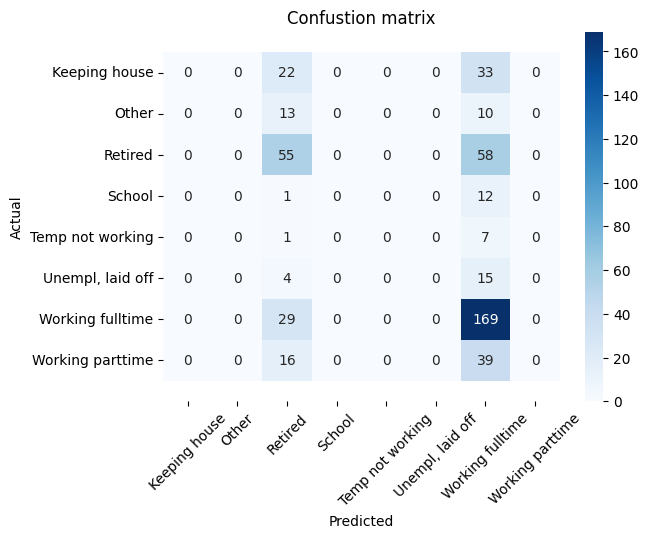
\includegraphics[width=0.6\textwidth]{figures/Thanh/Models/MLP_Deep_Learning/With_null_models_confusion_matrix_MLP_original_features.png}
    \caption{Ma trận nhầm lẫn của mô hình MLP khi vector đầu vào là vector gốc ban đầu}
    \label{fig:With_null_models_confusion_matrix_MLP_original_features}
\end{figure}

Cũng như trường hợp tập dữ liệu chỉ bao gồm các quan sát có cột emailtotal không phải null ta nhận thấy kết quả phân loại không khác biệt hay nổi trội hơn các mô hình trước.
Điều này cũng phản ánh sự khó phân biệt của phân phối dữ liệu tương ứng với từng nhãn trong cột wrkstat.
